\chapter{Trajectory Generation Pipeline}
\label{cha:concepts}
In this chapter, the pipeline to generate trajectories for mobile subscribers is introduced. The developed pipeline consists of a five-steps model, which is shown in Figure~\ref{fig:pipeline}. The concept to generate trajectories is the following: The input data is iteratively used to generate trajectories for each subscriber. The output is a trajectory which consists of the route, traveled by the subscriber, as well as timestamps, which defines the point in time when the subscriber was located at this location. Given below each step of the pipeline is described in more detail to better understand how the system operates.
\begin{figure}
	\centering
	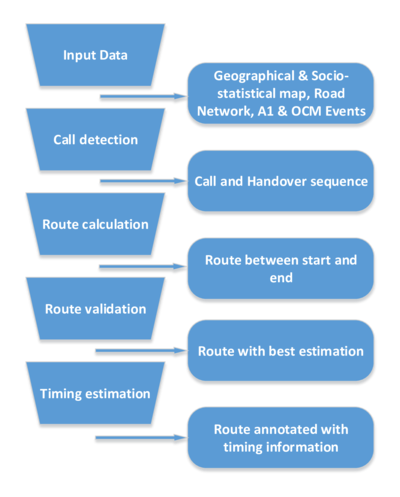
\includegraphics[width=0.7\linewidth]{./images/pipeline}
	\caption{Developed trajectory generation pipeline. The trapezoids represent the single steps in the pipeline, the rounded rectangles illustrate the
	outputs of the particular steps}
	\label{fig:pipeline}
\end{figure}
\section{Input Data}
This section focuses on input data that are consumed by the system. The gathering of input data is the first step in the developed pipeline. Moreover input data can be distinguished between four data types, which are used by the system: geographical data, socio-statistical data, mobile subscription data (A1 and OCM), road network data. The different data types are described in the succeeding sections.
\subsection{Geographical Input Data}
As mentioned before GSM does not expose an accurate location of the subscriber. In GSM, only the Cell-ID of the current connected cell is known. However, to calculate a route between the start and end of the call a more accurate location is needed. Because the coverage area of cell can be from as little as  $500m^2$ up to $50km^2$, boundaries need to be set in which subscribers can be located. The assumption is that the majority of subscribers will start or end their journey in an urban fabric whereas only a small fraction of subscribers will start or end their journey in open land.
In the course of this project the geographic information is derived from data from the \emph{CORINE}\footnote{CORINE: "Coordination of Information on the Environment"; \url{http://www.eea.europa.
eu/publications/COR0-landcover}, last accessed on March 11,2014} project which was initiated by the European Commission in 1985. The main purpose of this project was to generate a geographic information system for the member states of the European Union.
The \emph{CORINE} land cover (CLC) project is one essential part of the \emph{CORINE} projects which aims to develop a land cover information system for twelve member states of the European Union (Effective 2006). The \emph{CORINE} land cover project distinguishes between five main categories and in total 44 land cover classes. Out of the five only two categories are applicable for the purpose of defining boundaries where a subscriber can be located: \emph{artificial surfaces} and \emph{agricultural areas}. The three remaining categories --\emph{forest
	and semi-natural areas}, \emph{wetlands} and \emph{water bodies}-- can be considered as areas where subscribers are not starting or ending their calls.
The \emph{CORINE} land cover data for Austria can be obtained from the following service\footnote{\url{http://www.data.gv.at/datensatz/?id=9246f37d-da69-4442-9504-ebd006a059bb},
	last accessed on March 11,2014}. The land cover data is provided in two different data types, first as a raster image with a grid size of 100 meters and second as a Shapefile. Figure~\ref{fig:clc_austria} illustrates the land cover map\footnote{Image source: \url{http://www.eea.europa.eu/data-and-maps/figures/corine-land-cover-2000-by-country/clc00_at_national.eps/image_original}l, last accessed on March 11,2014.} of Austria. The red spots within the image represents urban fabric areas whereas green denotes to forest and semi-natural areas.
\begin{figure}
	\centering
	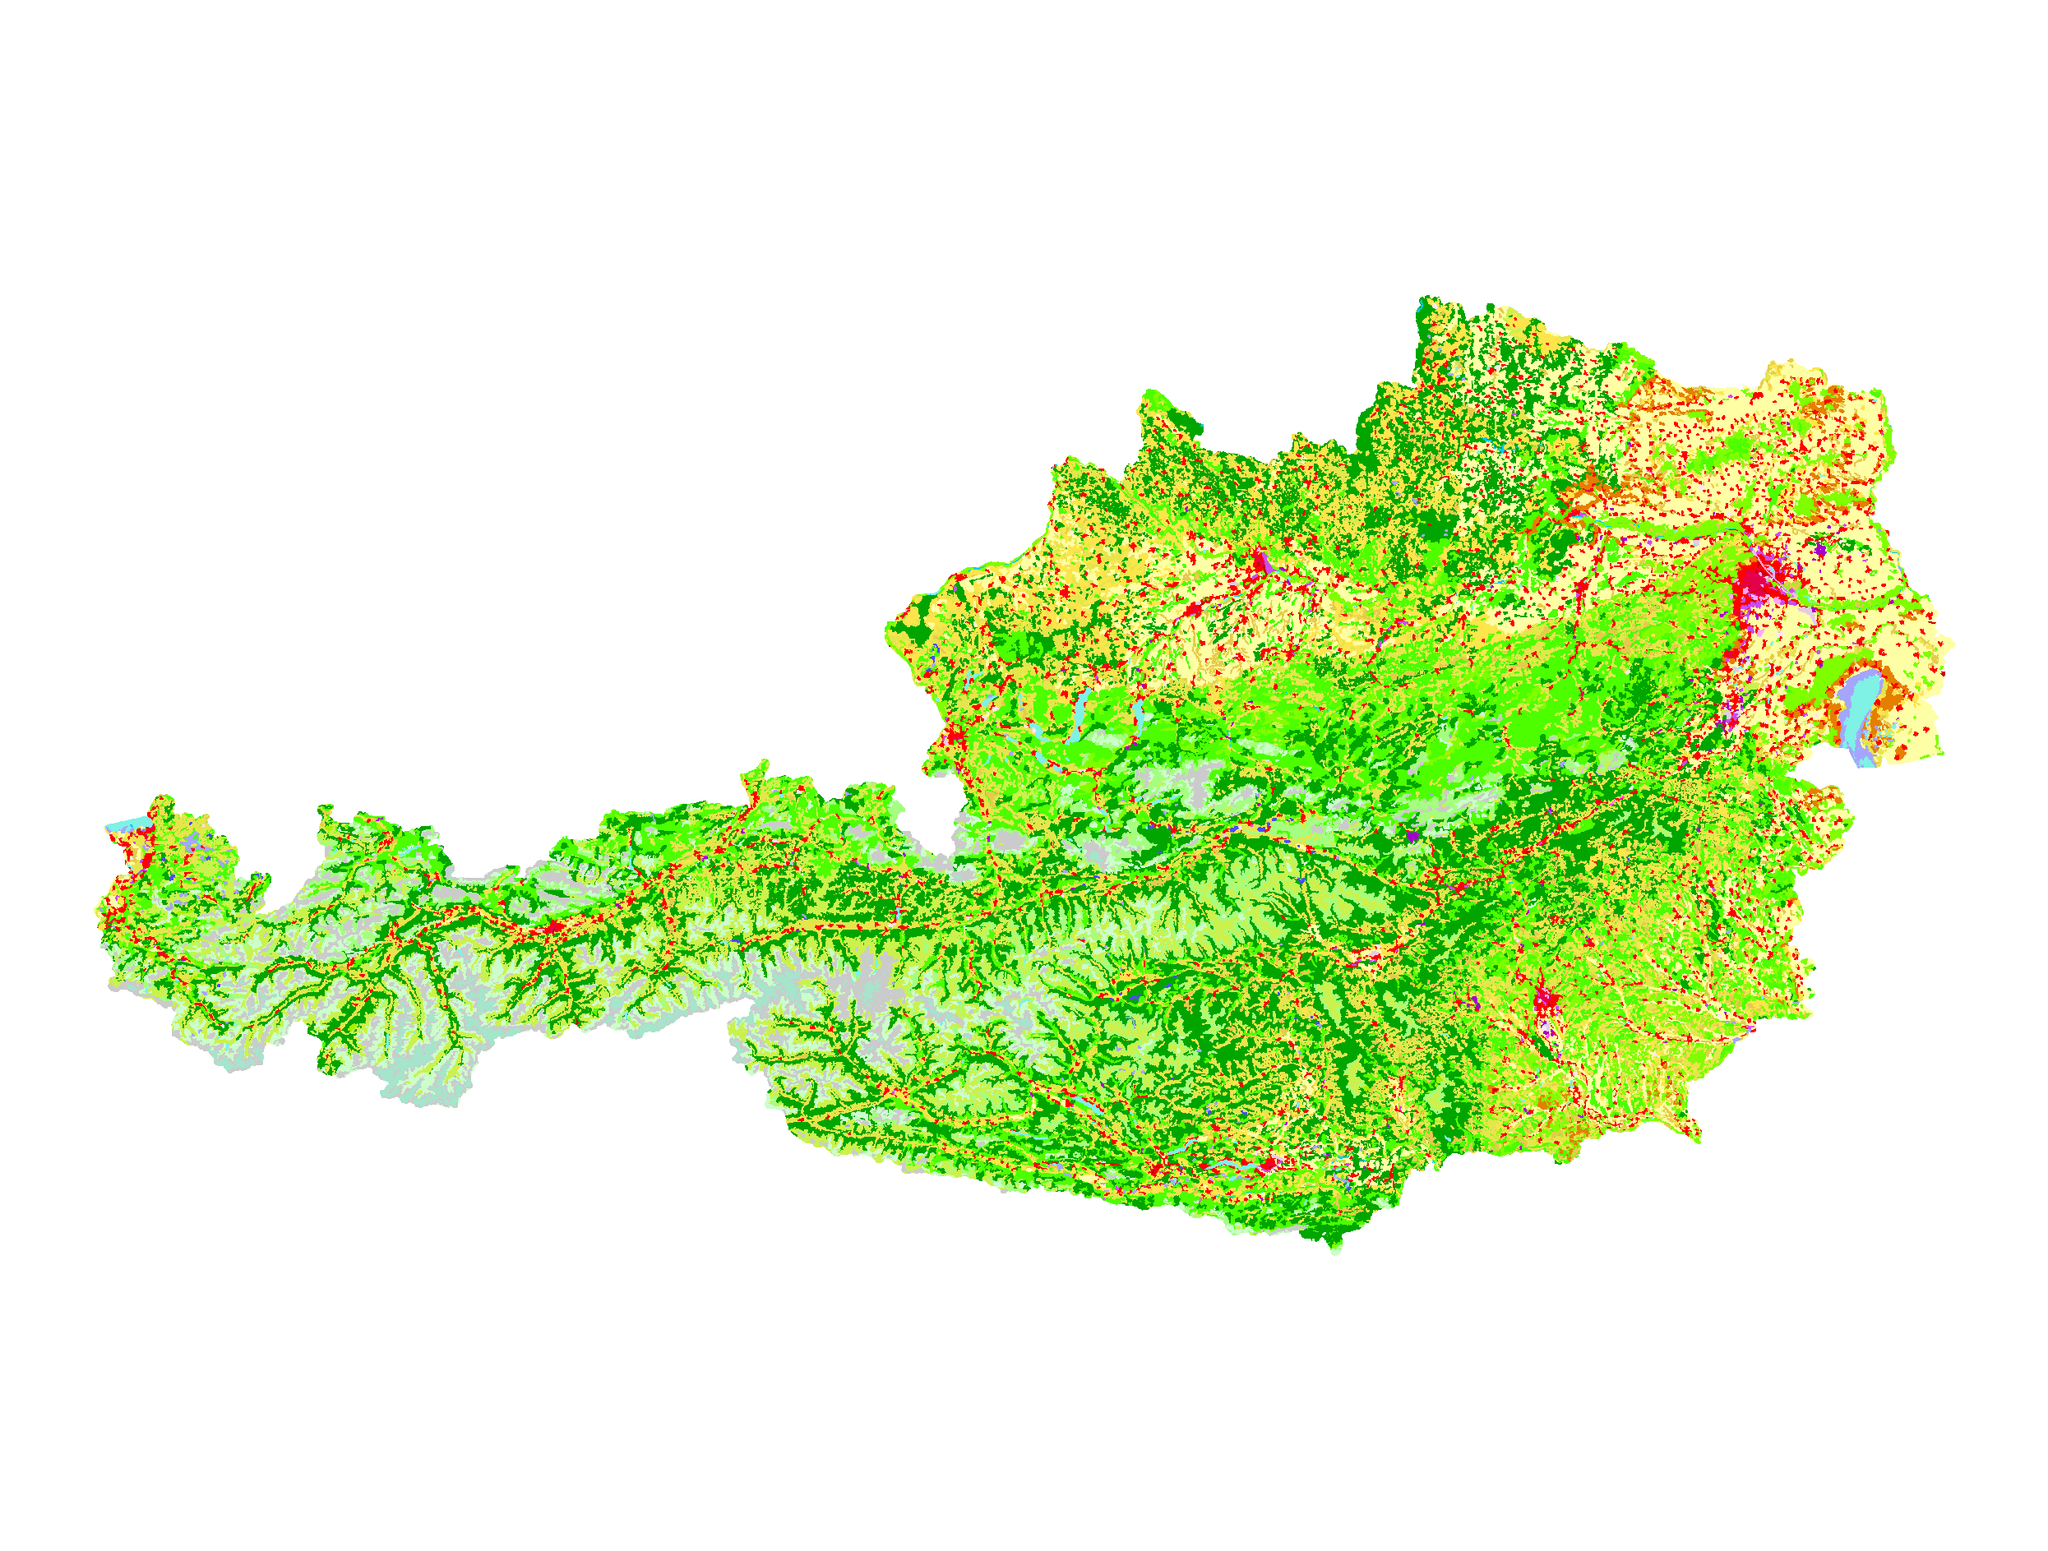
\includegraphics[width=\linewidth]{./images/clc_austria.png}
	\caption{Corine land cover map of Austria}
	\label{fig:clc_austria}
\end{figure}

\subsection{Socio-statistical Input Data}
The second type of input data used in the generation pipeline are population density maps. Population density maps belong to the class of socio-statistical maps and provide information about the distribution of population in a geographical area. Gallego et al.~\cite{Gallego2010,Gallego2011} describe several disaggregation methods which can be used to generate a population density map of the European Union.
Their approach uses information from the \emph{CORINE} land cover project to derive a population density grid with 100 meters grid spacing. The population density grid is used in the developed system to narrow the location of a user within the current connected cell. This works in conjunction with \emph{CORINE} land cover. A more detailed description of the described process will be presented later.
The population density grid can be obtained freely from the European Environment Agency (EEA) \footnote{\url{http://www.eea.europa.eu/data-and-maps/data/population-density-disaggregated-with-
	corine-land-cover-2000-2}, last accessed on March 11,2014}. Similar to the \emph{CORINE} land cover data the population density grid is available in two data types.
	\subsection{Road Network}
	The last input data for the developed system is a representation of the road network. Individuals walk or drive on predefined paths: streets, paths, etc. To generate trajectories, the system needs to have a representation of the road network to assign the path of subscribers on the road network. A freely available and open-source road network is provided by the OpenStreetMap\footnote{\url{http://www.openstreetmap.org/about}, last accessed on March 12, 2014} project. The aim of OpenStreetMap is to provide a world wide map which can be used without any royalties. Contributers all over the world are feeding OpenStreetMap with new data. Therefore, OpenStreetMap is very accurate for locations where the number of contributers is high. Figure~\ref{fig:map_linz} illustrates a map\footnote{Image source: \url{http://render.openstreetmap.org/cgi-bin/export?bbox=14.278879165649414,48.31028478774528,14.302825927734377,48.320590159843626&scale=5754&format=pdf}, last accessed on March 12, 2014} of Linz, Austria generated by OpenStreetMap. It can be seen that OpenStreetMap provides a large variety of data (e.g.\ streets, paths, buildings, POI, etc.).
	
	The developed system utilizes the road network from OpenStreetMap to estimate a start and end position of the trajectory as well for route generation. Additionally OpenStreetMap is used to validate the timing estimation for subscribers where no GPS path is available which is the case for A1 subscribers.
	\begin{figure}
		\centering
		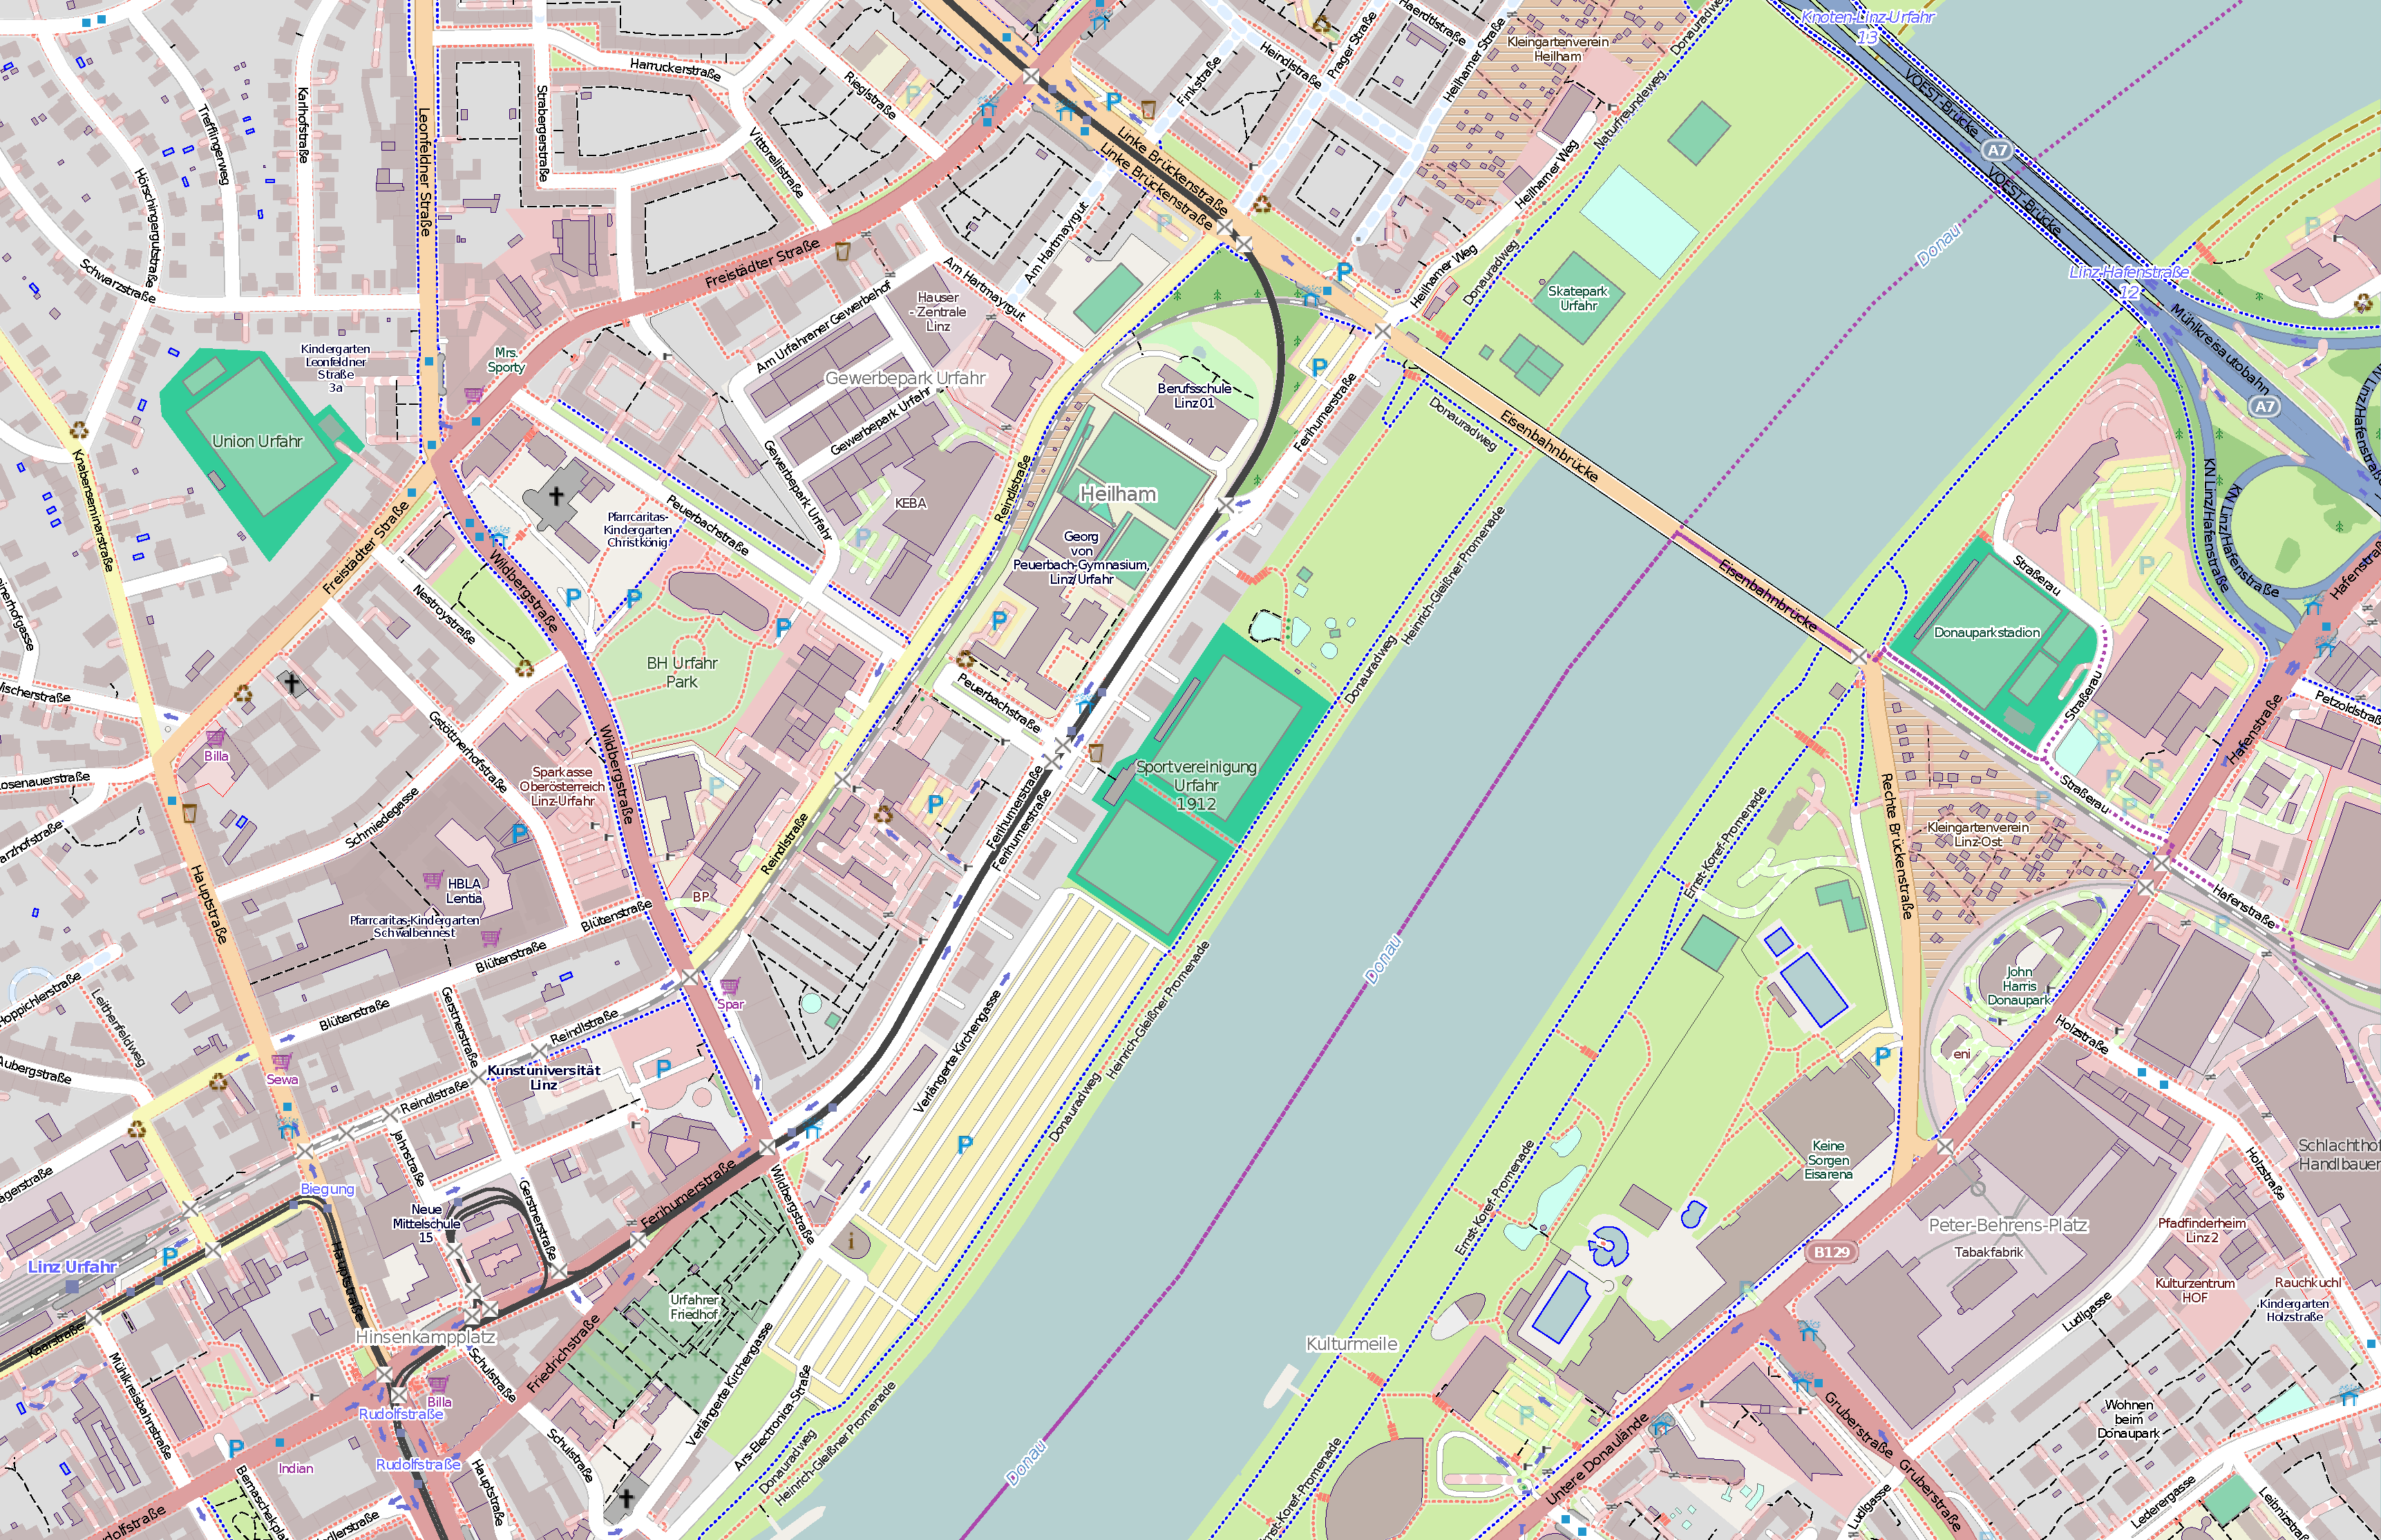
\includegraphics[width=0.7\linewidth]{./images/map_linz}
		\caption{OpenStreetMap map of a part of Linz, Austria}
		\label{fig:map_linz}
	\end{figure}
\subsection{Subscriber Information}
\subsubsection{A1 Dataset}
The mobile subscription data which is provided by A1 is used to generate trajectories for subscribers. To generate trajectories, the developed system is fed with an event stream for a special user. This event stream contains all events which have been captured during one day. As we mentioned before in Section~\ref{sec:anonymous} the anonymous user id changes at least every 24 hours. Therefore it is only possible to extract trajectories for one day per subscriber. Each event stream can contain zero, one or $n$ calls. Every call in the event stream represents a trajectory.
\subsubsection{OCM Dataset}
In order to validate our approach we need not only an event stream but also the path traveled by the subscriber. Therefore, the developed system uses an event stream provided by the OpenCoverageMap project. After a conversion to the A1 event format, this event stream can be provided to the developed system. In addition to the A1 event stream, it contains the traveled path which was recorded via GPS on a mobile phone. The GPS tracks allow the system to validate the route finding process as well as the timing estimation. The comparison between the estimated trajectory and the actually traveled route helps to validate the routing. By calculating the speed from the GPS the system can validate how well the timing estimation has been done. More details to the validation process will be provided in Section~\ref{sec:routevalidation},\ref{sec:timing-estimation}.

\subsection{Network Coverage}
\subsubsection{Voronoi Coverage}
The developed system needs a representation of the coverage area for each cell site. As described before in Section~\ref{sec:voronoites} Voronoi tessellation can be used to calculate an approximate coverage area. However, as Voronoi tessellation only takes the location of the cell site and not the physical characteristics (shadowing, antenna gain, reflections, path loss,etc.\ ) the approximation is not very accurate. To calculate the coverage area --the Voronoi polygon -- for each cell site, the system is using the location and the angle of the antenna as input data for the calculation. The angle is needed to separate sector antennas which are mounted on the same cell tower.
\subsubsection{Coverage Prediction}
Because the developed system is based on handover point estimation, an accurate approximation of the coverage area is needed. Besides Voronoi tessellation, a network planning tool is used. The network planning tool not only takes the location of the cell site but also the physical characteristics into account. Characteristics taken into account by the network planning tool are:
\begin{itemize}
	\item Digital Elevation Model
	\item Transmit Power
	\item Path Loss
	\item Shadowing
	\item Line Of Sight
	\item Multi-path propagation
\end{itemize}
By using the physical characteristics, the calculated coverage area is more accurate than the simple approximation done with Voronoi tessellation. Since this system has no access to the physical properties of the operator, it is using freely available information. This information consists of a Digital Elevation Model of the research area and the transmit power of cell sites.
\paragraph{Digital Elevation Model}
The network planning tool is using a Digital Elevation Model to calculate properties such as path loss, shadowing and line of sight. This properties are important for the coverage prediction. The European Environment Agency\footnote{Data source: \url{http://www.eea.europa.eu/data-and-maps/data/ds_resolveuid/ca503256de1b4231b029e4145d0a8b7b} last accessed March 19, 2014} provides a Digital Elevation Model of Europe. A Digital Elevation Model is aligned in a grid and for each cell of the grid the altitude above sea level is known. The EEA Digital Elevation Model consists of a raster with 25 meters grid spacing. The quality of the coverage prediction is limited by the resolution of the underlying Digital Elevation Model. Therefore by using a better model the accuracy of the prediction can be increased.
\paragraph{Transmit Power}
The transmit power defines the power level of the transmitter of the antenna. An increase in transmit power Since an increase in coverage since the path loss effect will be minimized. Because the network operator has not provided any information about the transmit power of its BTS the system is using an alternative data source. In Austria the Forum Mobilkommunikation provides a service called \emph{Senderkataster}\footnote{Project description: \url{http://www.senderkataster.at/} last accessed March 19, 2014}. The Senderkataster allows to view all broadcast and mobile communication transmitters on a map. In addition to the location it, also depicts the transmit power range. The Senderkataster defines the following four categories for transmit power:
\begin{itemize}
	\item Category 1: < 15 Watt
	\item Category 2: 15 - 50 Watt
	\item Category 3: 50 - 100 Watt
	\item Category 4: > 100 Watt
\end{itemize}
By querying the Senderkataster with the research area, the system can get the transmitting power. However, the Senderkataster is a voluntary project and relies on the data provided by mobile network operators. This has the disadvantage that not every cell site of a network operator is listed in the Senderkataster.
\paragraph{Data Extraction}
The Senderkataster service can be queried with simple HTTP requests (see Listing~\ref{lst:senderbbox}). The services takes a bounding box of the research area and returns all transmitters withing the bounding box. The bounding box is defined by the four parameters --left, right, bottom, top -- \emph{EXL}, \emph{EXR}, \emph{EXB} and \emph{EXT}. The coordinates are projected in the WIGeoEU projection (EPSG 7397) \footnote{Projection string: \url{http://spatialreference.org/ref/sr-org/7397/html/} last accessed March 19, 2014}. After the request was sent to the service, the service delivers all the transmitters in the following format \lstinline+301377|314876|2057165+. The first parameter is the internal ID of the transmitter, second the X coordinate, and lastly the Y coordinate. The ID can then be used to retrieve additional informations such as the transmitting power, the transmitter type and if it is mounted on a house or a tower.

To retrieve more information about the transmitter a request (see Listing~\ref{lst:transmitterinfo}) to the service with the ID is made. The response to the request is the following: \lstinline+mobilfunk|301377|GSM/UMTS|d|41,48|1+ . The first parameter describes the transmitter, it can either be a mobile radio network or a broadcast transmitter used for terrestrial radio and television . Second is the ID, the third one depicts the used technology (GSM, GPRS, UMTL, LTE), the fourth indicates if the transmitter is mounted on the roof (d) or a tower (e), followed by the transmit power in Watt and the last parameter shows if other transmitter are using the same tower.
\begin{lstlisting}[caption=Request to retrieve station within the boudning box,label=lst:senderbbox]
http://www.senderkataster.at/functions/getPoints.php5
?EXL=312790.83396198
&EXR=315119.16603802
&EXB=2056054.8754715
&EXT=2057801.1245285
\end{lstlisting}

\begin{lstlisting}[caption=Request to retrieve transmitter information,label=lst:transmitterinfo]
http://www.senderkataster.at/functions/getInfos.php5
?TYPE=mobilfunk
&ID=301377
\end{lstlisting}
\paragraph{Cell Site and Transmitter Position}
The latitude and longitude coordinates of the A1 data specify the location of the cell tower. On each cell tower there can be one or more transmitters mounted. The network planning tool is using two databases, one for the cell site (tower position) and the second one for transmitters. Each transmitter is assigned to one cell site whereas a cell site can be connected to one or more transmitters.

By querying the A1 data set and only storing unique tuples of latitude and longitude, the system can derive all cell site locations. To get the transmitters for each cell site, the A1 data set is queried for each unique location tuple. A basic transmitter consists of a location, Cell-ID, LAC, transmit power, height and angle. The location is a direct relation to the cell site. The power indicates the transmit power of the transmitter. As there is not information about the installment height of the transmitter it was set to be $20$ meters for all transmitters. A higher transmitter height might increase the coverage area for areas shadowed by hills or buildings. The angle defines the mounting angle and indicates in which direction the transmitter is beaming.

\paragraph{Best Server Plot}
All the above mentioned data is fed into the network planning tool to calculate the best server plot that is used as a coverage prediction. A best server plot calculates the path-loss effect for each transmitter. The path-loss specifies the reduction of power density of an electromagnetic wave as it propagates through space. To calculate the path loss for each transmitter the COST-Hata model is used which extends the urban Okumura-Hata model~\cite{,Laiho2006,Mishra2007,Ghasemi2011}. The  main equations of the COST-Hata model are depicted in Equation~ \ref{eq:costhata}.
\begin{dgroup}
\label{eq:costhata}
\begin{dmath}
\label{eq:pathloss}
L \; = \; 46.3 \; + \; 33.9\log f \; - \; 13.82 \log h_B \; - \; a(h_R) \; + \; [44.9 \;- \;6.55 \log h_B] \log d \; + \; C
\end{dmath}
\begin{dmath}
\label{eq:antennacor}
a(h_R)\;=\;(1.1\log f\;-\;0.7)h_R\;-\;(1.56\log f\;-\;0.8)
\end{dmath}
\begin{dmath}
C \; = \; \begin{cases} 0 \; dB \mbox{  for medium cities and suburban areas} \\ 3 \; dB \mbox{  for metropolitan areas} \end{cases}
\end{dmath}
\begin{dsuspend}
$L$ = Median path loss. Unit: Decibel (dB)

$f$ = Frequency of Transmission. Unit: Megahertz (MHz)

$hBl$ = Base Station Antenna effective height. Unit: Meter (m)

$d$ = Link distance. Unit: Kilometer (km)

$hR$ = Mobile Station Antenna effective height. Unit: Meter (m)

$a(hR)$ = Mobile station Antenna height correction factor as described in the Hata Model for Urban Areas..
\end{dsuspend}
\end{dgroup}

The path loss was calculated for various distance in the interval [0..5000] meters. Therefore, the path loss effect for each transmitter in the calculation area is known. The coverage prediction simply takes the path loss effect and assigns the best server as the transmitter with the least path loss.

\begin{figure}
	\centering
	\begin{subfigure}[b]{0.45\textwidth}
		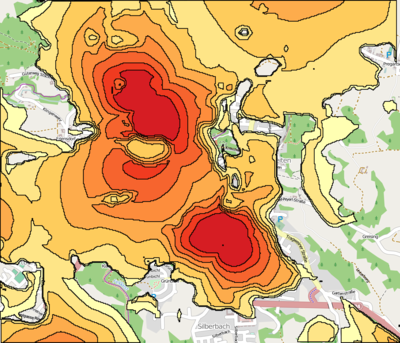
\includegraphics[width=\textwidth]{./images/signallevelmapsmall}
		\caption{Signal Level Plot}
		\label{fig:signallevel}
	\end{subfigure}%
	~ %add desired spacing between images, e. g. ~, \quad, \qquad etc.
	%(or a blank line to force the subfigure onto a new line)
	\begin{subfigure}[b]{0.45\textwidth}
		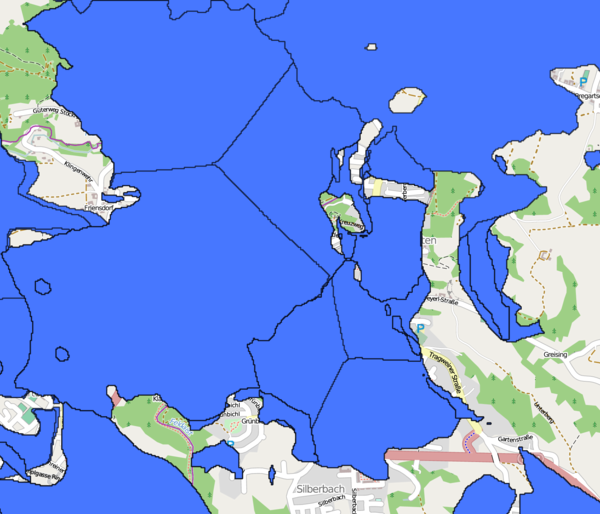
\includegraphics[width=\textwidth]{./images/coveragemapsmall}
		\caption{Coverage Prediction}
		\label{fig:coveragepred}
	\end{subfigure}
\begin{subfigure}[b]{\textwidth}
		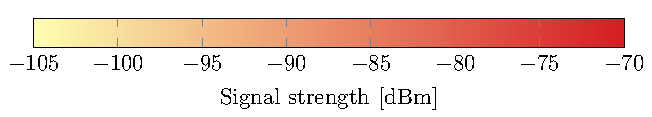
\includegraphics[width=\textwidth]{./images/signallevelbar}
		\caption{}
		\label{fig:signallevelbar}
	\end{subfigure}



	\caption{A signal level plot (a) with its signal strength (c) and a coverage prediction for Hagenberg, Austria }
	\label{fig:cellarea}
\end{figure}

Figure~\ref{fig:cellarea} shows two different path-loss plots for Hagenberg, Austria. The first one Figure~\ref{fig:signallevel} depicts the attenuation for each transmitter in the area. The red area indicates a small attenuation whereas yellow indicates a high attenuation. The colorbar in Figure~\ref{fig:signallevelbar} indicates the signal strength (dBm) for the above signal level plot.

%\begin{center}
%\tikzsetnextfilename{signallevelbar}
%\begin{tikzpicture}
%
%\begin{axis}[
%    hide axis,
%    scale only axis,
%    height=0pt,
%    width=0pt,
%    colormap={yellowred}{ rgb255(0cm)=(255,255,178); rgb255(1cm)=(214,29,35)},
%    colorbar horizontal,
%    point meta min=-105,
%    point meta max=-70,
%    colorbar style={
%        width=10cm,
%        xtick={-105,-100,-95,-90,-85,-80,-75,-70},
%        xlabel={Signal strength [dBm]}
%    }]
%    \addplot [draw=none] coordinates {(0,0)};
%\end{axis}
%\end{tikzpicture}
%\end{center}
From theses attenuation values, a best server plot -- coverage prediction -- for each transmitter can be derived as shown in Figure~\ref{fig:coveragepred}. It can be seen that there is an overlapping area between neighboring transmitters. The system is using the predicted coverage area for start and end point estimation and timing purposes.



\section{Call Detection}
This section describes the process of filtering calls within each event stream. The two used event streams -- A1 and OCM -- are using different events to signalize call establishment and termination. After this process, the system can generate a trajectory for each call found in the event stream.
\paragraph{A1 Calls}
To signalize the establishment of a call in the A1 event stream either a \emph{Mobile Originated Call} or a \emph{Mobile Terminated Call} event is issued. The first event is used when a mobile station initiates a call with another subscriber. The mobile station of the other subscriber will issue the second event once the call has been established with the first subscriber.

When either of the involved subscribers terminates the call, a \emph{A Disconnect} event shall be issued by both subscribers. However, during an investigation of the event stream there was no occurrence of this event. Therefore the developed system is using an approach by which it investigates events that have been issued after a call establishment. If the system recognizes either one of the following events: \emph{SMS}, \emph{Mobile Originated Call}, \emph{Mobile Terminated Call}, \emph{Location Area Update} or \emph{IMSI detach} it generates a call termination event before.

\paragraph{OCM Calls}
Rather than capturing events in the network, the OpenCoverageMap project periodically stores the state of the mobile phone. The state can either be \emph{idle} or \emph{connected}. In order to detect a call, the system has to find changes in the state. If a state change is detected the corresponding event is issued. A call establishment is detected when the state changes from \emph{idle} to \emph{connected}. In contrast to the call establishment, the call termination is detected when the state changes from \emph{connected} to \emph{idle}.

The detection of call terminations is more accurate for OpenCoverageMap than for A1 where no information is available if a call is still ongoing. Because OpenCoverageMap periodically stores the state of the mobile phone whereas in order to detect a call termination for A1 events the system has to recognize a follow-up event.

\section{Route Calculation}
The following section presents the process of calculating a route for a mobile subscriber. In general each call is used to calculate one route which is later transfered to a trajectory. The process consists of several steps which will be described in the succeeding sections.
\subsubsection{Start and End Position Estimation}
\label{sec:startandend}
The first step in the route calculation process is to estimate the subscribers start and end position. As mentioned before GSM only exposes the Cell-ID which only defines a boundary in which the subscriber is located. To narrow this boundaries the system is using geographical input (\emph{CORNINE} land cover) and socio-statistical maps (population density maps).

By using \emph{CORNINE} land cover data the system can define areas where it is unlikely that a subscriber will start or end his journey. This step can be parameterized by giving each of the CLC classes a percentage factor. The percentage defines how likely it is that a subscriber starts or ends a call in this class.

Our second assumption is that subscribers will more likely start or end their call in a higher populated area within the cell boundaries. More subscribers are located in higher populated areas than in less populated ones. Therefore the system is using population density maps in order to better estimate the start or end position. Figure~\ref{fig:pop_vienna} shows an example for a population density map for Vienna, Austria. In this example it can be seen that the density is higher in the inner districts than in the outer ones.
\begin{figure}
	\centering
	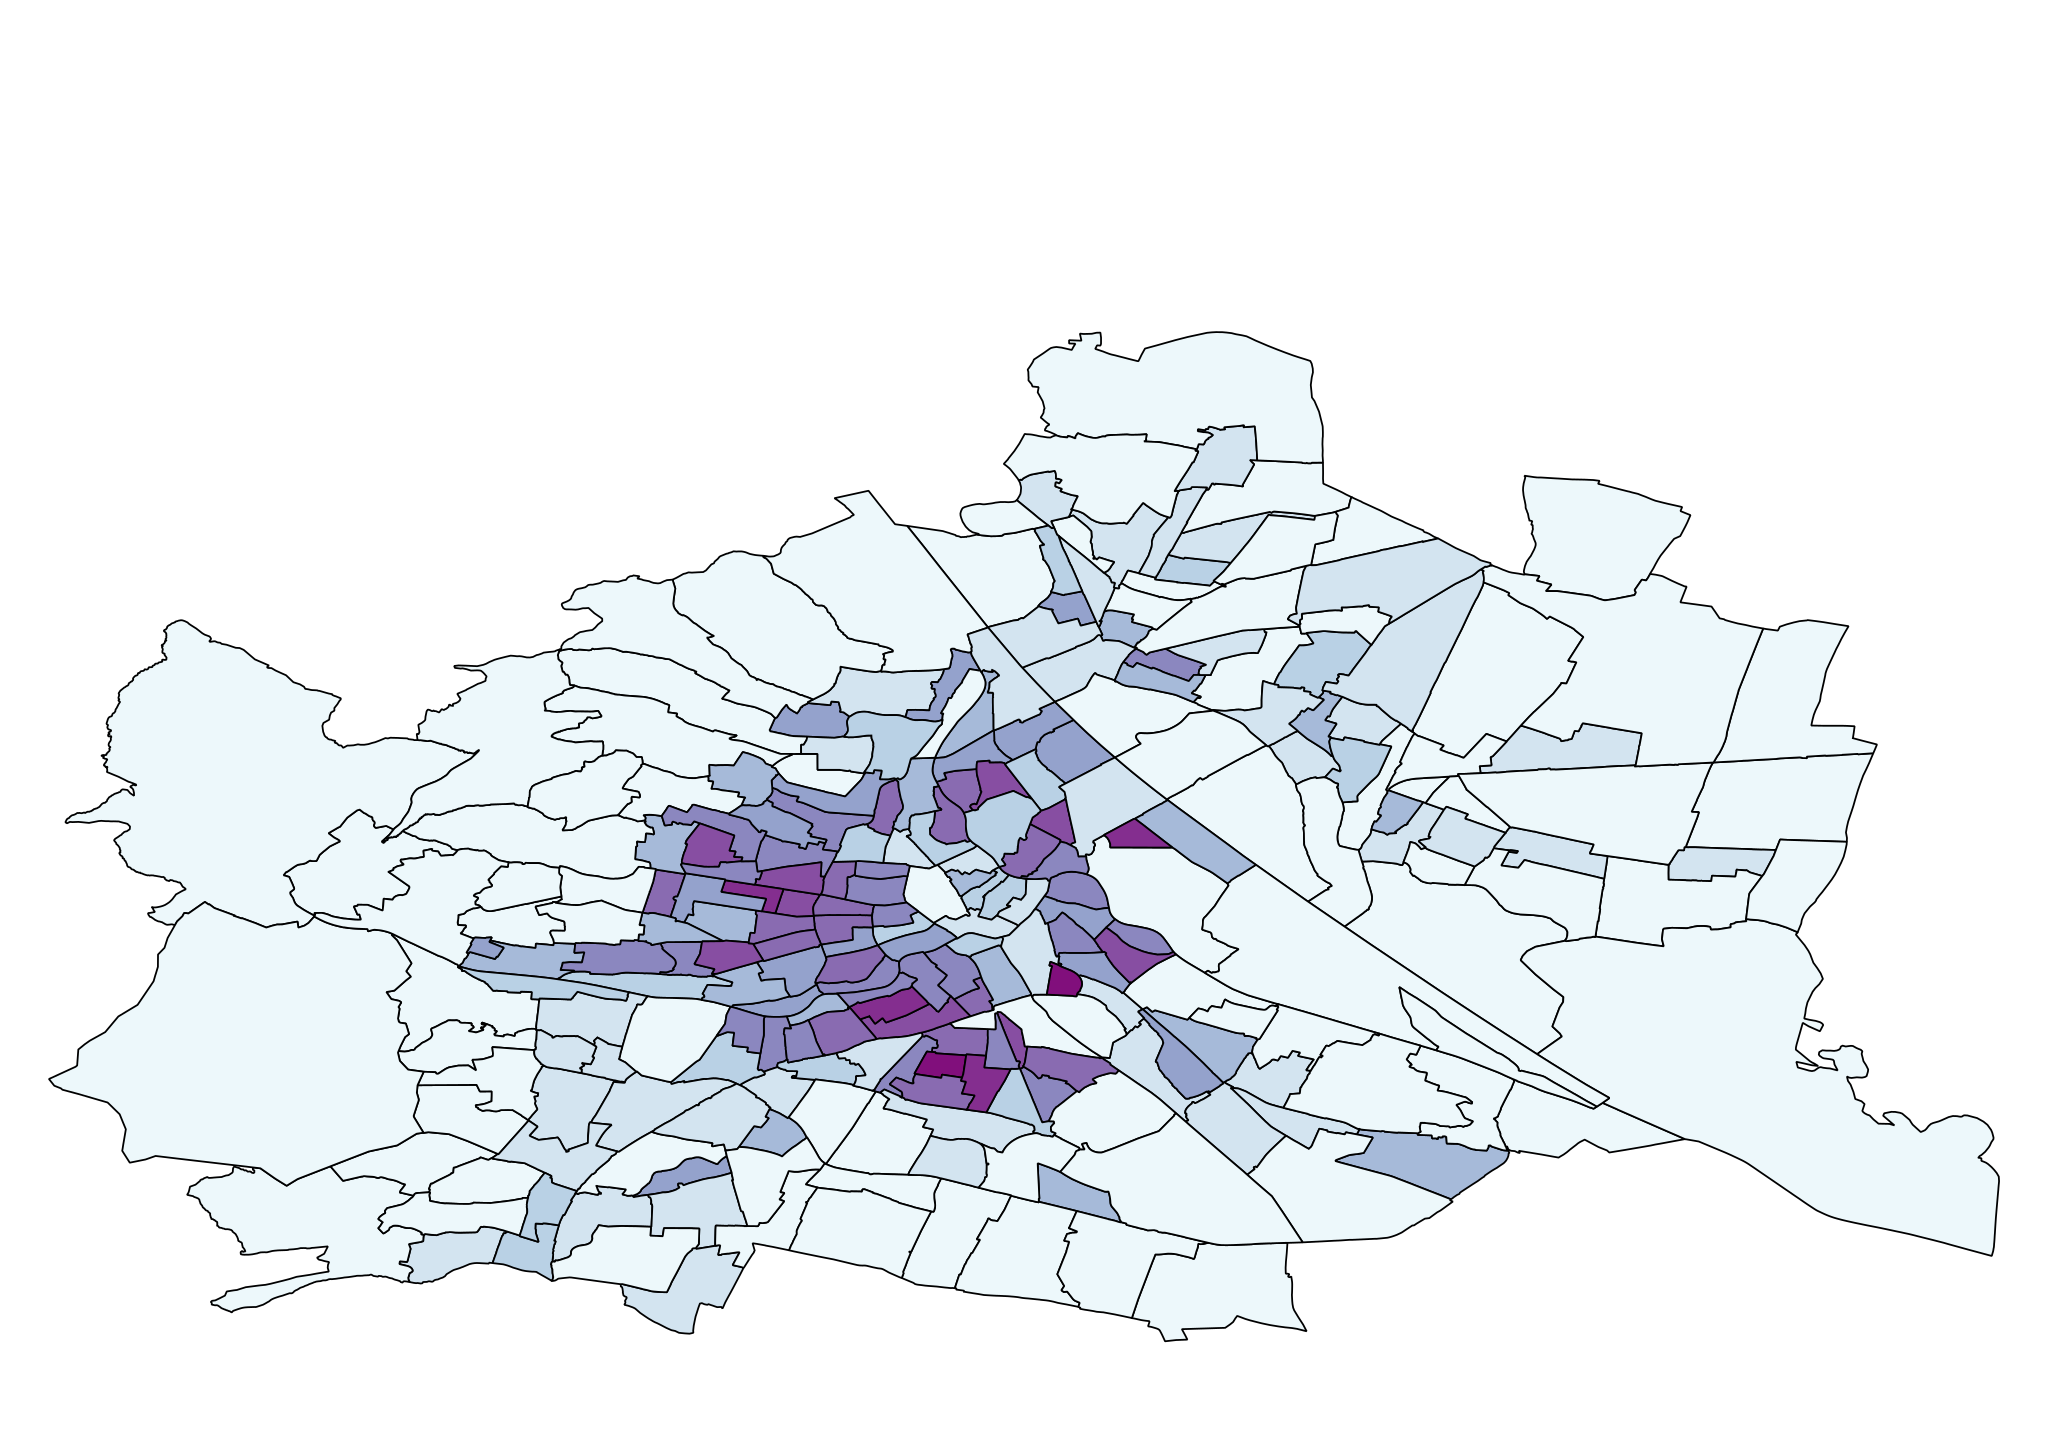
\includegraphics[width=0.7\linewidth]{./images/pop_vienna}
	\caption{Population density map of Vienna, Austria. The population density is higher in darker (purple) than in brigher areas}
	\label{fig:pop_vienna}
\end{figure}
\subsubsection{Corine Land Cover Clipping}
By clipping and therefore removing unwanted areas the system can narrow the boundaries in which a subscriber is located. To clip the coverage area of a cell the system loads the \emph{Corine} land cover map for the particular area. The next step is to clip the cell coverage area with useful \emph{CORINE} land cover categories such as \emph{artificial surfaces} and \emph{agricultural areas}. This technique known as polygon clipping removes unwanted area --\emph{forest and semi-natural areas}, \emph{wetlands} and \emph{water bodies} -- from the cell.
%Afterwards a \emph{Corine} land cover class is picked by the system based on the percentage given to each. By creating a probability density function for a random number generator \emph{Corine} land cover classes can
\subsubsection{Population Density Estimation}
After removing unwanted areas within the cell coverage area the next step is to estimate the subscribers position. This step is the same for start and end positions. By using the population density information of the coverage area the system dices a position based on the population density. Therefore more subscribers will be located in higher populated areas.

\paragraph{Population Density Clipping}
The first step is to load the population density map for the coverage area. A random number generator with a defined probability density function will be created. The probability density function is derived from the population density map. When the system loads the population density map for the coverage area it will get $n$ polygons with $n$ different population densities. More generally speaking each area with a unique population density is represented by a polygon. Afterwards the random number generator is used to dice an area of interest. By using the population density as a function for the random number generator, areas with a high population density will be picked more often than less populated areas. Once the system picked a polygon based on the random number generator it clips this polygon with the coverage area. This process narrows the boundaries of the subscribers location. Following the subscribers location will be set by dicing a location within the remaining coverage area. Figure~\ref{fig:population} illustrates an example for different population densities within the boundaries of one cell. We can see that the total population is $315$. We calculate a \emph{pdf} for all three population cells based on the ratio of the population and the total population. The calculated \emph{pdf} will be used to estimate the user's start and end position. As an example the probability that the starting point is within the polygon with Population $240$ is given by $240$/$315$. Within the polygon ``Population 240'' the starting point is selected based on a uniform distribution.
\begin{figure}

	\centering
	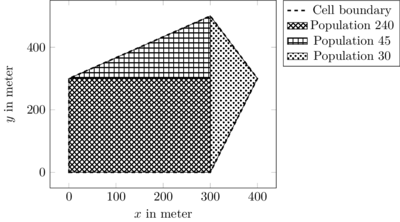
\includegraphics[width=\columnwidth]{./images/population_cell}
%	\tikzsetnextfilename{population}
%	\begin{tikzpicture}[scale=0.70]
%		\begin{axis}[
%				xlabel=$x$ in meter,
%				ylabel=$y$ in meter,
%			legend pos=outer north east]
%
%			\addplot+[mark=none,draw=black, very thick,dashed] coordinates
%			{(0,0) (300,0) (400,300) (300,500) (0,300)} -- cycle;
%			\addlegendentry{Cell boundary}
%
%			\addplot+[mark=none,pattern=crosshatch,area legend,draw=black] coordinates
%			{(0,0) (300,0) (300,300) (0,300)} -- cycle;
%			\addlegendentry{Population 240}
%
%			\addplot+[mark=none,pattern=grid,area legend,draw=black] coordinates
%			{(0,300) (300,300) (300,500) (0,300) } -- cycle;
%			\addlegendentry{Population 45}
%
%			\addplot+[mark=none,pattern=crosshatch dots,area legend,draw=black] coordinates
%			{(300,0) (300,500) (400,300) }-- cycle;
%			\addlegendentry{Population 30}
%
%
%
%		\end{axis}
%	\end{tikzpicture}

	\caption{A Demonstration of a Population Grid for a Cell Area}
	\label{fig:population}
\end{figure}

\paragraph{Random Point in Coverage Area}
Dicing a random location into a rectangular shape is an easy task, however the shape of the remaining coverage area will unlikely be a rectangular. A simple approach is using the bounding box of the coverage area polygon and dicing coordinate pairs for the bounding box as long as one coordinate pair lays within the coverage polygon. This simple approach has one major disadvantage because it is unpredictable. There is no estimation for how long it would take that one coordinate pair is contained in the coverage polygon.

A more sophisticated approach is to triangulate the coverage polygon into triangles. Triangulation of convex monotype polygons can be done with algorithms by A. Fournier and D.Y. Montuno~\cite{Fournier1984} or Godfried Toussaint~\cite{Toussaint1984}. The developed system uses the GDAL project~\cite{GDAL} which provides an implementation of polygon triangulation for many platforms and programming languages.
Figure~\ref{fig:triangulation} depicts the triangulation of a polygon into triangles. The polygon is split into 3 triangles by applying Fourniers algorithm.

\begin{figure}

	\centering
	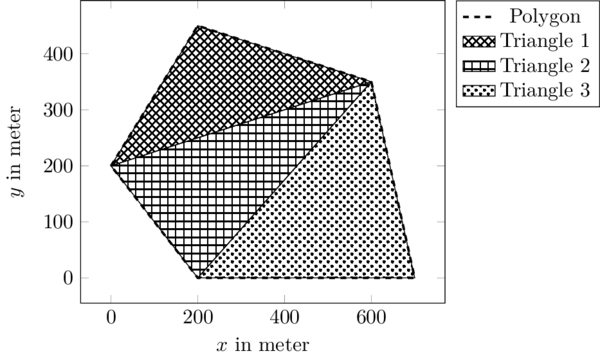
\includegraphics[width=\columnwidth]{./images/population_poly}
%	%\tikzsetnextfilename{population2}
%	\begin{tikzpicture}[scale=0.70]
%		\begin{axis}[
%				xlabel=$x$ in meter,
%				ylabel=$y$ in meter,
%			legend pos=outer north east]
%
%			%    \addplot+[mark=none,draw=black, very thick,dashed] coordinates
%			%		{(0,0) (300,0) (400,300) (300,500) (0,300)} -- cycle;
%			%    \addlegendentry{Cell boundary}
%
%			\addplot+[mark=none,draw=black, very thick,dashed] coordinates
%			{(0,200) (200,450) (600,350)(700,0)(200,0) } -- cycle;
%			\addlegendentry{Polygon}
%			\addplot+[mark=none,pattern=crosshatch,area legend,draw=black] coordinates
%			{(0,200) (200,450) (600,350) } -- cycle;
%			\addlegendentry{Triangle 1}
%			\addplot+[mark=none,pattern=grid,area legend,draw=black] coordinates
%			{(0,200)  (600,350)(200,0) } -- cycle;
%			\addlegendentry{Triangle 2}
%			\addplot+[mark=none,pattern=crosshatch dots,area legend,draw=black] coordinates
%			{(200,0)  (600,350)(700,0) } -- cycle;
%			\addlegendentry{Triangle 3}
%			%	\addlegendentry{Polygon}
%
%
%			%   	\addlegendentry{Population 240}
%
%
%
%		\end{axis}
%	\end{tikzpicture}

	\caption{Triangulation of a Polygon into 3 Triangles}
	\label{fig:triangulation}
\end{figure}
As already discussed before the developed system needs to uniformly distribute subscribers location with the polygon. A \emph{pdf} will be created by using the area of each triangle as input. A random number generator will use this \emph{pdf} and randomly assign the triangle in which the subscribers location shall be diced.

In Figure~\ref{fig:comprandom} two different approaches for random triangle point picking are illustrated. The first one is picking a point within the boundaries of the triangle whereas the second one is picking a point in a  quadrilateral which consist of the triangle and its mirroring. To pick a point in a triangle the first approach is using Equation~\ref{eq:randtriangle} where $a_1$ and $a_2$ are uniform random numbers in the interval $ \left[0,1 \right] $, $v_1$ and $v_2$ are two vertices's of the triangle. As depicted in Figure~\ref{fig:randtriangle} this approach does not create uniform distributed points within the triangle. The second approach is different from the first one as it does not pick points within the triangle but rather in a quadrilateral made of the original triangle and its mirroring. Figure~\ref{fig:quadrilateral} shows that this approach creates uniform distributed points. However the points are created in a quadrilateral instead of a triangle this can be overcome by removing points outside of the triangle. Since our system needs a uniform distribution of points in a triangle, the second approach will be used.
\begin{equation}
	p=a_1*v_1+(1-a_1)*a_2*v_2
	\label{eq:randtriangle}
\end{equation}

\begin{equation}
	p=a_1*v_1+a_2*v_2
	\label{eq:randquad}
\end{equation}


\begin{figure}
	\centering
	\begin{subfigure}[b]{0.45\textwidth}
		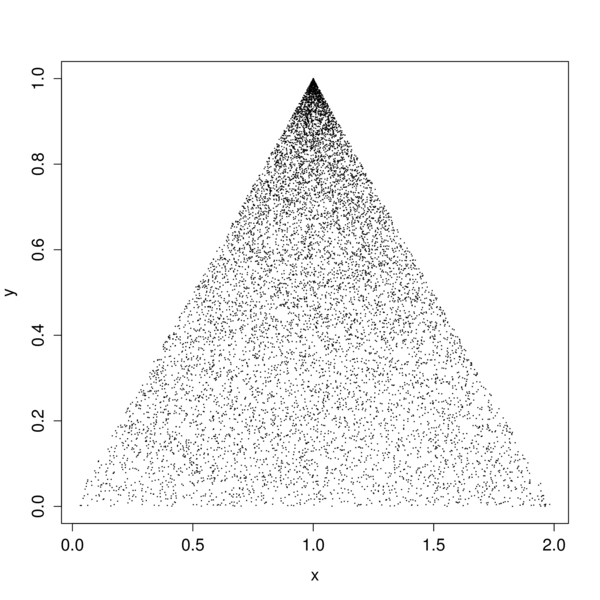
\includegraphics[width=\textwidth]{./images/randompointpolygon}
		\caption{Random Point in Triangle}
		\label{fig:randtriangle}
	\end{subfigure}%
	~ %add desired spacing between images, e. g. ~, \quad, \qquad etc.
	%(or a blank line to force the subfigure onto a new line)
	\begin{subfigure}[b]{0.45\textwidth}
		
\includegraphics[width=\textwidth]{./images/randompointquadliteral}
		\caption{Random Point in  Quadrilateral}
		\label{fig:quadrilateral}
	\end{subfigure}

	\caption{Comparison between two different random point picking methods}
	\label{fig:comprandom}
\end{figure}

\subsubsection{Routing}
The developed system is using the OpenStreetMap road network and the OSM2PO\footnote{Project description: \url{http://osm2po.de/}, last accessed on March 18,2014} route engine. After estimating a random start and end position of the subscriber a route between these two points will be calculated with OSM2PO.

\paragraph{OSM2PO}
OSM2PO is a project developed by Carsten Moeller which allows routing on the freely available OpenStreetMap road network. On the first start OSM2PO is generating a graph network out of the road network. The graph network is used internally of OSM2PO and allows a faster route calculation. OSM2PO can calculate the fastest route by using speed limit information or the shortest route with minimum distance.
\paragraph{Route Generation}
The system first estimates a start and position for the subscriber and calculates the fastest route between these two points. The calculated route contains the geometry of the route, the used roads and the speed limit of each road segment. This information will later be used by the system to validate the route.
\section{Route Validation}
\label{sec:routevalidation}
Route validation is necessary to use the best estimation of the traveled route. For each subscriber there will be more than one route generated based on a configuration parameter. The developed system uses two different types of route validation, the first evaluates the route geometry and the second the timing. Each of the validations can be treated separately or in conjunction. By combining the results a better validation can be achieved.
\subsubsection{Geometry Validation}

Geometry validation is used to evaluate the estimated route with the subscribers handover sequence. In addition when using events from the OpenCoverageMap the system can validate the estimated route with the actual route based on the GPS information.
\paragraph{Squared Sum}
The first validation the system is doing for each route is to calculate the squared sum between the cell sites of the handover sequence and the calculated route. To compare different routes Equation~\ref{eq:sumsquaremine} was used. This is the same metric Tettamanti et al.\cite{Tettamanti2010} used for their system. For each calculated route $j$ the squared sum of all minimum distances $d_{i,j}$  between the route and the cell site was calculated. Figure~\ref{fig:rms} illustrates the minimum distance between the centroid of a cell site and a calculated route.

\begin{equation}
	\label{eq:sumsquaremine}
	D_j=\sum_{i=1}^{m} d_{i,j}^{2}
\end{equation}
%\begin{equation}
%\label{eq:minsummine}
%min(D_j), j = 1,2,\ldots,n
%\end{equation}
\begin{figure}
	\centering
	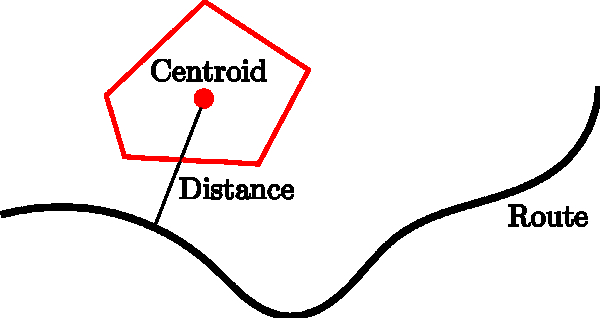
\includegraphics[width=0.7\linewidth]{./images/rms}
	\caption{Minimum distance between centroid of cell site and route}
	\label{fig:rms}
\end{figure}


\paragraph{Hausdorff Distance}
If the system is using events from the OpenCoverageMap project the actual route traveled by the subscriber is known by storing GPS information. This allows the system to validate the calculated routes with the actual route. The developed system is using the Hausdorff distance named after Felix Hausdorff~\cite{Rockafellar1998}. The Hausdorff distance measures how far two subsets of a metric space are from each other, it is the maximum of all the distances from a point in one set to the closest point in the other set. In our system the two sets consists of the calculated and the actual route. Figure~\ref{fig:Hausdorff_distance_sample} depicts the Hausdorff\footnote{Image source: \url{http://en.wikipedia.org/wiki/File:Hausdorff_distance_sample.svg} last accessed on March 16, 2014 } distance between to paths $X$ and $Y$. Therefore the system is using the Hausdorff distance to measure the similarity between the calculated and the actual route.
\begin{figure}
	\centering
	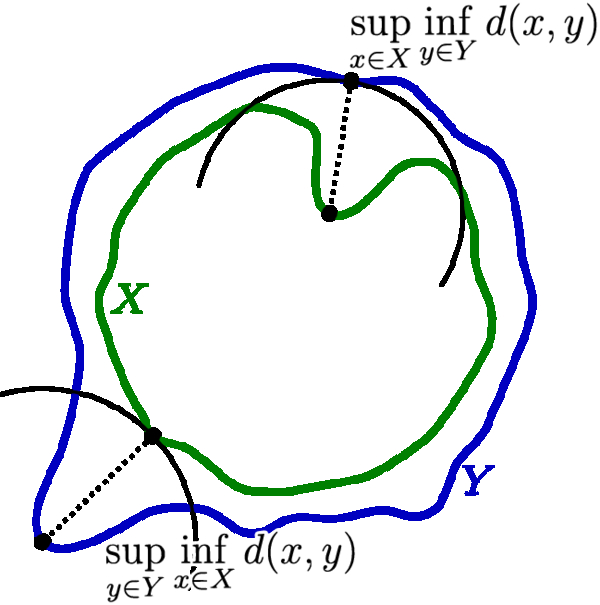
\includegraphics[width=0.7\linewidth]{./images/Hausdorff_distance_sample}
	\caption{Hausdorff distance between two sets}
	\label{fig:Hausdorff_distance_sample}
\end{figure}

\subsubsection{Timing Validation}
Besides geometry validation the system is taking the time it needs to actually drive the route into account. When the system generates a trajectory for a subscriber it knows the time when the subscriber initiated and terminated the call. This information is used to extract the journey time. A ratio $r_t$ between the actual journey time $t_{actual}$ and the time it takes to travel the estimated route $t_{route}$ is calculated (see Equation~\ref{eq:timeratio}). The ratio gives information if the estimated router is either to fast or to slow. A to fast route can indicate that the route is either too long or that the subscriber was stuck in traffic congestions. On the other hand a slower estimated route can indicate that either the wrong route was chosen or that the subscriber was going faster than the speed limit. Therefore a conjunction of all validations is needed to choose the best approximated route.
\begin{equation}
	r_{t}=\frac{t{actual}}{t{route}}
	\label{eq:timeratio}
\end{equation}

\section{Timing Estimation}
\label{sec:timing-estimation}
Whenever a subscriber is in an active call and moves from one cell to another one a handover event is issued. This event exposes a coarse location and a time stamp. By using this information the system can derive the velocity of the subscriber. The velocity of a subscriber is an important figure for mobility simulation. Because the velocity together with the estimated route describes the mobility of the subscriber. However as we the system only knows the cell in which the handover event originated -- cell to which handover was made -- an estimation of the actual handover point is needed. A more precise estimation of this handover point results in a better velocity approximation.
\subsubsection{Handover Position Estimation}
To estimate handover points the system is using two successive handover events. These two events consists of a time stamp, cell-Id and LAC. From the cell-Id and LAC the system can obtain the coverage area of the two cells. During research of the A1 and OCM data we discovered that there are two types of handover. The successive handover are either connected or apart. Connected handover are handover which coverage areas touches or overlaps each other. An apart handover is a handover where the coverage areas are not touching or overlapping.
\begin{figure}
	\centering
	\begin{subfigure}[b]{0.4\textwidth}
		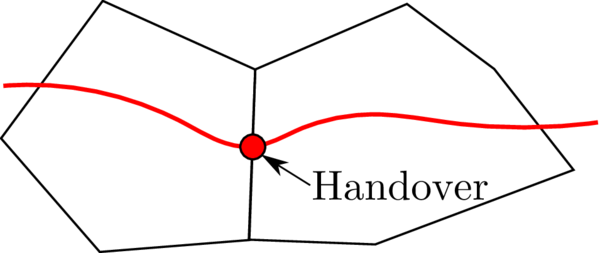
\includegraphics[width=\textwidth]{./images/handover_together}
		\caption{}
		\label{fig:handovertogether}
	\end{subfigure}%
	~ %add desired spacing between images, e. g. ~, \quad, \qquad etc.
	%(or a blank line to force the subfigure onto a new line)
	\begin{subfigure}[b]{0.55\textwidth}
		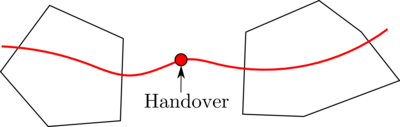
\includegraphics[width=\textwidth]{./images/handover_apart}
		\caption{}
		\label{fig:handoverapart}
	\end{subfigure}

	\caption{Example for connected (a) and apart (b) handover}
	\label{fig:handovertypes}
\end{figure}
The difference of the two handover types is illustrated in Figure~\ref{fig:handovertypes}. For connected handover it is obvious where the handover happened. For this purpose the system is taking the touching or overlapping parts of the coverage areas and the intersection with the estimated route. In contrast for apart handover it is not clear where the handover happened. It could either happen at the boundaries of the first cell or the second cell or in between those. A simplification is to use the middle point between the two cells.
\subsubsection{Velocity}
\label{sec:velocity}
After the handover points have been estimated the next step is to enrich this information with the timestamps when the handover occurred. As mentioned before in Section~\ref{subsec:events} each event contains a precise timestamp when the event was captured by the underlying system. This information together with an estimated route and handover point allows to derive the velocity of the driver. The system knows the time difference between two handover events as well as the distance traveled. The traveled distance is the distance between two successive handover points. By cutting the whole route with the two handover points the system can obtain the route between the two handover points and therefore the actual distance between those. The velocity can then be calculated  by dividing the distance $s$ between the handover over the time difference $t$ between the handover $v=\frac{s}{t}$. The calculated velocity represents the average distance between the handover.
\subsubsection{Velocity Adaption}
\label{sec:adaption}
The handover position approximation is a static process and does not take the current situation into account. Therefore, it cannot react to dynamic events. This events can be high network load or short-term obstacles that affect the path loss of the transmitter. Since it is not feasible to get an accurate approximation of the coverage area for each cell site, the handover position can be error-prone. This can lead to a deviation of the exact handover position and the estimated one. To minimize this effect the handover position needs to be repositioned in case the estimate velocity is too high. An example for such an adaption is to move the handover position on the route. 
A deviation between the exact handover position and the approximated can lead to a higher or a lower average velocity. If the average velocity of one route segment is relative high, then there must exist another route segment with a relative low average velocity. We defined a rule that if the average calculated velocity of a route segment is greater than $50\%$ of the allowed maximum velocity a reposition takes place.  
Repositioning is done by first calculating the distance a subscriber can move from one handover time-stamp $H_i$ to the next one $H_{i+1}$, considering the allowed maximum velocity. The handover point $H_{i+1 }$ is then repositioned so that the distance between $H_i$ and $H_{i+1}$ equals the allowed distance. By decreasing the distance between $H_i$ and $H_{i+1}$ the distance between $H_{i+1}$ and $H_{i+2}$ will increase. This leads to a velocity decrease for the route segment between $H_i$ and $H_{i+1}$ and a velocity increase for $H_{i+1}$  and $H_{i+2}$.

An example for a handover repositioning is shown in Figure~\ref{fig:1058handoveradapted}. The green points are the handover positions observed by the handset. In contrast, the blue points are the estimated handover points. Handover were estimated with the above presented approach. The example illustrates that the second estimated handover is too far from the observed one away. Here a handover is made to a cell whose coverage the subscriber has not yet entered. Therefore, the above presented approach estimated a wrong handover position based on the assumption that; handovers happen at the edge of coverage cells. 

\begin{figure}
\centering
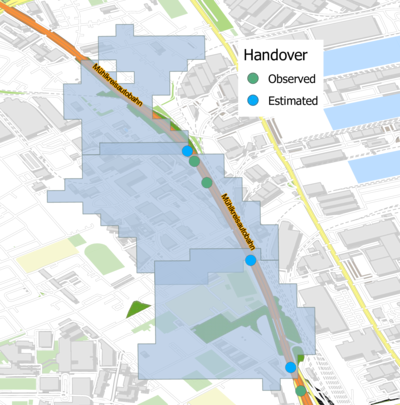
\includegraphics[width=0.7\linewidth]{./images/1058handoveradapted}
\caption{Derivation between the observed handover position and the estimated handover position}
\label{fig:1058handoveradapted}
\end{figure}

This leads to a deviation between those handover points that resulted in an average route segment (i) velocity of 396 km/h (see Figure~\ref{fig:1058adaptioncomp}). On the other hand the route segment (i+1) velocity of the successive segment was only 44 km/h due to the increased route segment length. By applying the reposition algorithm the velocity of the route segment (i) was decreased to 80 km/h. The velocity of the other route segment (i+1) was increased to 77 km/h. 
 
While investigating the benefit of handover reposition we discovered that in some cases it is necessary to not only reposition one handover point but two. This needs to be done if the velocity transition from one route segment to another would lead to a high velocity of the second route segment. In such cases it is necessary to equally move the handover (i-1) and handover (i+1). Generally speaking this means that the velocity overrun from route segment (i) will be equally distributed over route segment (i-1) and (i+1).


\begin{figure}
\centering
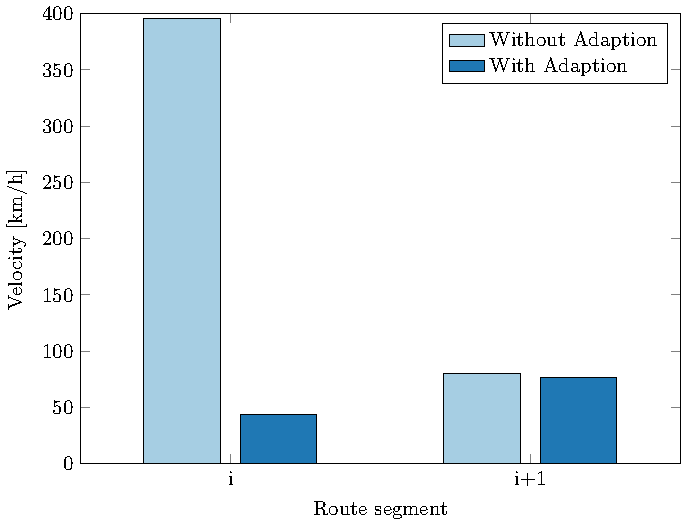
\includegraphics[width=0.7\linewidth]{./images/1058adaptioncomp}
%\definecolor{mycolor1}{rgb}{0.65098,0.80784,0.89020}%
%\definecolor{mycolor2}{rgb}{0.12157,0.47059,0.70588}%
%%
%\tikzsetnextfilename{1058adaptioncomp}
%\begin{tikzpicture}
%
%\begin{axis}[%
%width=4in,
%height=3in,
%area legend,
%scale only axis,
%xmin=0.5,
%xmax=2.5,
%xtick={1,2},
%xticklabels={{i},{i+1}},
%xlabel={Route segment},
%ymin=0,
%ymax=400,
%ylabel={Velocity [km/h]},
%legend style={draw=black,fill=white,legend cell align=left}
%]
%\addplot[ybar,bar width=0.513103448275862in,bar shift=-0.320689655172414in,draw=black,fill=mycolor1] plot table[row sep=crcr] {%
%1	396\\
%2	80\\
%};
%\addlegendentry{Without Adaption};
%
%\addplot [color=black,solid,forget plot]
%  table[row sep=crcr]{0.5	0\\
%2.5	0\\
%};
%\addplot[ybar,bar width=0.513103448275862in,bar shift=0.320689655172414in,draw=black,fill=mycolor2] plot table[row sep=crcr] {%
%1	44\\
%2	77\\
%};
%\addlegendentry{With Adaption};
%
%\end{axis}
%\end{tikzpicture}%

\caption{Comparison between the velocity without adaption and with adaption}
\label{fig:1058adaptioncomp}
\end{figure}